\section{Optimizasyon Teorisine Giriş}
Optimizasyon teorisi, bir sistemin performansını belirli kısıtlar altında en iyi duruma getirmeyi amaçlayan matematiksel ve metodolojik yaklaşımların bütünüdür. Bu ders, yapısal sistemlerin optimizasyonuna odaklanarak, temel kavramları ve uygulama yöntemlerini ele alacaktır.

\subsection{Optimizasyonun Tanımı ve Mühendislikteki Önemi}
Optimizasyon, bir sistemin performansını belirli kısıtlar altında en iyi duruma getirme sürecidir. \sidenote{Günlük hayatta sıkça karşılaştığımız "en iyi" kararı verme süreçleri aslında birer optimizasyon problemidir. Örneğin, işe giderken en kısa yolu seçmek, market alışverişinde en uygun fiyatlı ürünleri tercih etmek gibi.} Bu süreç, mühendislik tasarımlarında maliyeti düşürürken performansı artırmayı hedefler.


\subsection{Yapısal Optimizasyonun Temel Bileşenleri}
Yapısal optimizasyon, üç temel bileşen üzerine kurulur: amaç fonksiyonu, tasarım değişkenleri ve kısıtlar. Bu bileşenler, optimizasyon probleminin matematiksel formülasyonunu oluşturur.

\begin{itemize}
    \item \textbf{Amaç Fonksiyonu:} Minimize veya maksimize edilmek istenen hedef (örn. ağırlık, maliyet, rijitlik)
    \item \textbf{Tasarım Değişkenleri:} Optimize edilecek parametreler (örn. kesit boyutları, malzeme özellikleri)
    \item \textbf{Kısıtlar:} Tasarımın sağlaması gereken koşullar (örn. gerilme limitleri, deplasman sınırları)
\end{itemize}

\begin{marginfigure}
\centering
\begin{tikzpicture}
\draw[->] (0,0) -- (4,0) node[right] {$x_i$};
\draw[->] (0,0) -- (0,3) node[above] {$F(x)$};
\draw[scale=1,domain=0.5:3.5,smooth,variable=\x,blue] plot ({\x},{2.5*exp(-0.5*(\x-2)^2)});
\draw[red,dashed] (2,0) -- (2,2.5);
\filldraw[red] (2,2.5) circle (2pt) node[above] {Optimum};
\end{tikzpicture}
\caption{Tek değişkenli bir optimizasyon probleminde optimum noktanın gösterimi}
\label{fig:single_var_opt}
\end{marginfigure}

\subsection{Optimizasyonun Tarihçesi ve Gelişimi}
Optimizasyon teorisinin temelleri, matematiksel analiz yöntemlerinin gelişimiyle paralel olarak ilerlemiştir. Modern optimizasyon yöntemleri, bilgisayar teknolojisinin gelişimiyle birlikte yeni boyutlar kazanmıştır. \sidenote{İlk yapısal optimizasyon çalışmaları, Michell'in 1904'te yayınladığı kafes sistemlerin minimum ağırlık tasarımı ile başlamıştır. Bu çalışma, modern topoloji optimizasyonunun temelini oluşturur.}

\subsubsection{Önemli Tarihsel Gelişmeler}
\begin{itemize}
    \item 1940'lar: Doğrusal programlama ve Simplex metodunun geliştirilmesi
    \item 1950'ler: Dinamik programlama ve konveks optimizasyon teorisi
    \item 1960'lar: Sonlu elemanlar yönteminin optimizasyona uygulanması
    \item 1970'ler: Sayısal optimizasyon algoritmalarının geliştirilmesi
    \item 1980'ler: Metasezgisel algoritmaların ortaya çıkışı
    \item 1990'lar: Topoloji optimizasyonunun yaygınlaşması
    \item 2000'ler: Çok amaçlı optimizasyon ve yapay zeka tekniklerinin entegrasyonu
\end{itemize}

\subsection{Optimizasyon Problemlerinin Genel Yapısı}
Her optimizasyon problemi, bir amaç fonksiyonunun minimizasyonu veya maksimizasyonu şeklinde ifade edilir. Problem formülasyonu, tasarım değişkenlerini ve kısıtları içerir. \sidenote{Optimizasyon probleminin matematiksel formülasyonu, problemi sistematik bir şekilde çözebilmemiz için gerekli olan yapıyı sağlar. Bu formülasyon, farklı mühendislik problemlerini ortak bir çerçevede ele almamıza olanak tanır.}

\begin{equation}
\begin{aligned}
& \text{minimize} & & f(\mathbf{x}) \\
& \text{subject to} & & g_i(\mathbf{x}) \leq 0, & & i = 1,\ldots,m \\
& & & h_j(\mathbf{x}) = 0, & & j = 1,\ldots,p \\
& & & x_k^L \leq x_k \leq x_k^U, & & k = 1,\ldots,n
\end{aligned}
\end{equation}

\begin{tcolorbox}[title=Yapısal Optimizasyon Örneği]
Bir çelik kirişin optimum tasarımı için:
\begin{itemize}
    \item \textbf{Amaç:} Minimum ağırlık
    \item \textbf{Değişkenler:} Kesit yüksekliği ve genişliği
    \item \textbf{Kısıtlar:} 
        \begin{itemize}
            \item Maksimum gerilme $\leq$ Akma gerilmesi
            \item Maksimum sehim $\leq$ İzin verilen sehim
            \item Minimum kesit boyutları
        \end{itemize}
\end{itemize}
\end{tcolorbox}

\subsection{Optimizasyonun Mühendislikteki Temel Uygulama Alanları}
Optimizasyon, mühendisliğin çeşitli alanlarında yaygın olarak kullanılır. İnşaat, makine, havacılık ve uzay mühendisliği başlıca uygulama alanlarıdır.

\begin{itemize}
    \item \textbf{İnşaat Mühendisliği:}
        \begin{itemize}
            \item Çelik yapıların kesit optimizasyonu
            \item Betonarme elemanların donatı optimizasyonu
            \item Köprü tasarımında form optimizasyonu
        \end{itemize}
    \item \textbf{Makine Mühendisliği:}
        \begin{itemize}
            \item Mekanik parçaların şekil optimizasyonu
            \item Termal sistemlerin performans optimizasyonu
            \item Titreşim kontrolü ve sönümleme
        \end{itemize}
    \item \textbf{Havacılık ve Uzay Mühendisliği:}
        \begin{itemize}
            \item Kanat ve gövde tasarımı
            \item Kompozit malzeme optimizasyonu
            \item Yapısal ağırlık minimizasyonu
        \end{itemize}
\end{itemize}


\subsection{Deterministik ve Stokastik Optimizasyon Yaklaşımları}
Optimizasyon yöntemleri, problem çözme yaklaşımlarına göre deterministik \sidenote{Deterministik bir yöntemin, her çalıştırmada aynı sonucu vermesi gerektiği anlamına gelir. Yani stabil ve öngörülebilirdirler.} ve stokastik \sidenote{Stokastik ise bir yöntemin, her çalıştırmada farklı sonuçlar üretebilmesi gerektiği anlamına gelir. Yani rastgele ve öngörülemez (daha doğrusu öngörüsü kısıtlı) bir yöntemdir.} olmak üzere iki ana kategoriye ayrılır. 

\subsubsection{Deterministik Yaklaşımlar}
\begin{itemize}
    \item Her çalıştırmada aynı sonucu verir
    \item Gradyan tabanlı yöntemler bu kategoridedir
    \item Lokal optimuma takılma riski vardır
    \item Başlangıç noktasına bağımlıdır
\end{itemize}

\subsubsection{Stokastik Yaklaşımlar}
\begin{itemize}
    \item Rastgelelik içerir
    \item Her çalıştırmada farklı sonuçlar üretebilir
    \item Global optimumu bulma olasılığı daha yüksektir
    \item Genetik algoritmalar, tavlama benzetimi gibi yöntemler bu kategoridedir
\end{itemize}

Bu yaklaşımlar, farklı problem tiplerine uygun çözüm stratejileri sunar. \sidenote{Deterministik ve stokastik yaklaşımların seçimi, problemin yapısına ve çözüm gereksinimlerine bağlıdır. Örneğin, çok modlu bir problemde stokastik yöntemler daha avantajlı olabilir.}

\subsection{Doğrusal ve Doğrusal Olmayan Optimizasyon}
Optimizasyon problemleri, amaç fonksiyonu ve kısıtların yapısına göre doğrusal ve doğrusal olmayan problemler olarak sınıflandırılır. Bu sınıflandırma, kullanılacak çözüm yöntemlerini belirler.

\subsubsection{Doğrusal Optimizasyon}
\begin{itemize}
    \item Amaç fonksiyonu ve kısıtlar doğrusaldır
    \item Çözüm uzayı konvekstir
    \item Simplex metodu gibi etkin çözüm yöntemleri vardır
    \item Global optimum garanti edilir
\end{itemize}

\begin{tcolorbox}[title=Doğrusal Optimizasyon Örneği]
Bir üretim planlaması problemi:
\begin{equation*}
\begin{aligned}
\text{maximize} \quad & 3x_1 + 2x_2 \\
\text{subject to} \quad & 2x_1 + x_2 \leq 100 \\
& x_1 + x_2 \leq 80 \\
& x_1, x_2 \geq 0
\end{aligned}
\end{equation*}
\end{tcolorbox}

\subsubsection{Doğrusal Olmayan Optimizasyon}
\begin{itemize}
    \item Amaç fonksiyonu ve/veya kısıtlar doğrusal değildir
    \item Çözüm uzayı karmaşıktır
    \item Lokal optimumlar içerebilir
    \item Yapısal problemlerin çoğu bu kategoridedir \sidenote{Yapısal mühendislikte karşılaşılan problemlerin büyük çoğunluğu doğrusal olmayan karakterdedir. Örneğin, geometrik nonlineerite, malzeme nonlineeritesi gibi etkiler problemi doğrusal olmayan hale getirir.}
\end{itemize}

\begin{tcolorbox}[title=Doğrusal Olmayan Optimizasyon Örneği]
    Bir yapısal tasarım optimizasyonu problemi:
    \begin{equation*}
    \begin{aligned}
    \text{minimize} \quad & f(x) = x_1^2 + 2x_2^2 - 0.3x_1x_2 \\
    \text{subject to} \quad & g_1(x) = x_1^2 + x_2^2 - 25 \leq 0 \\
    & g_2(x) = x_1 - 2x_2 + 5 \leq 0 \\
    & -10 \leq x_1, x_2 \leq 10
    \end{aligned}
    \end{equation*}
    \end{tcolorbox}



\subsection{Çözüm Yöntemlerinin Genel Sınıflandırılması}
Optimizasyon yöntemleri, problem tipine ve çözüm stratejisine göre analitik, sayısal ve metasezgisel yöntemler olarak sınıflandırılır. Her yöntem grubu, belirli problem tipleri için avantajlar sunar.

\begin{itemize}
    \item \textbf{Analitik Yöntemler}
        \begin{itemize}
            \item Diferansiyel hesap
            \item Varyasyonel yöntemler
            \item Lagrange çarpanları
        \end{itemize}
    \item \textbf{Sayısal Yöntemler}
        \begin{itemize}
            \item Gradyan tabanlı yöntemler
            \item Doğrusal programlama
            \item Nonlineer programlama
        \end{itemize}
    \item \textbf{Metasezgisel Yöntemler}
        \begin{itemize}
            \item Genetik algoritmalar
            \item Parçacık sürü optimizasyonu
            \item Tavlama benzetimi
        \end{itemize}
\end{itemize}

\subsection{Optimizasyon Problemlerinde Global ve Lokal Optimumlar}

Çok modlu optimizasyon problemlerinde, birden fazla lokal optimum noktası bulunabilir. Bu durum, özellikle doğrusal olmayan problemlerde sıklıkla karşımıza çıkar.

\begin{figure}[H]
    \centering
    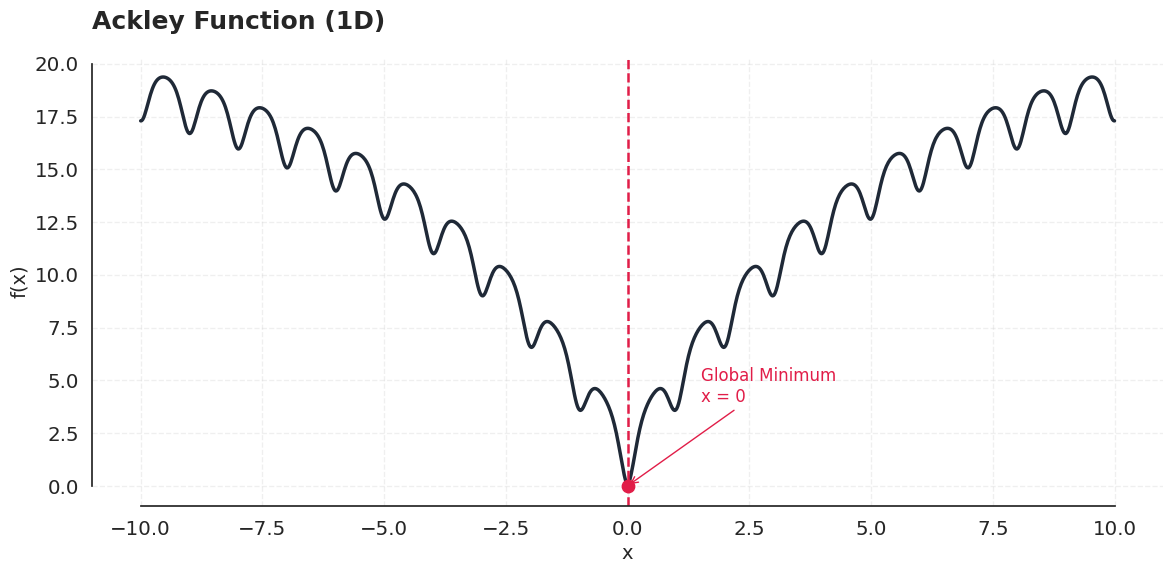
\includegraphics[width=\textwidth]{weeks_new/imgs/multi_mod.png}
    \caption{Tek boyutlu ve çok modlu optimizasyon problemi}
    \label{fig:multi_mod}
\end{figure}

Yukarıdaki şekilde görüldüğü gibi, çok modlu bir fonksiyonda birden fazla tepe (maksimum) ve çukur (minimum) noktası bulunabilir. Optimizasyon algoritmaları, başlangıç noktasına bağlı olarak lokal bir optimuma takılabilir ve global optimumu bulamayabilir. Bu nedenle, özellikle karmaşık mühendislik problemlerinde global optimumu bulmak için metasezgisel yöntemler tercih edilebilir.